
\section{Experimente mit ns-3-dev-TSCH}

Zur Analyse des Codes und des k"unftigen Anwendungsfall wurden mehrere Beispielscripte
erstellt um verschiedene Aspekte zu analysieren, welche nachfolgend erl"autert werden.

\subsection{Kommunikation und Scheduling}

Als Grundlage und Kernaufgabe wurde die normale Kommunikation innerhalb des TSCH
Mode definiert, wobei an ein solch erstelltes PAN mehrere Anfoderungen festgelegt wurden.

\begin{itemize}
  \item Star bzw. Mesh TSCH Netzwerk,
  \item 7 FFDs und 1 PAN-Coordinator,
  \item Slotframe Size von 8, wobei der erste Slot f"ur das Senden der
  EBs vom PAN-Coordinator festgelegt wird,
  \item 100 Bytes an Daten pro gesendetem Paket von jedem der FFDs zum
  PAN-Coordinator, wobei eine Fragmentierung der Pakete vermieden werden soll,
  \item kein Network-Formation,
  \item und das Network Scheduling ist beliebig, wobei Kollisionen und Shared-Slots
  auch vermieden werden.
\end{itemize}

F"ur die Topologie ist das bereits im vorherigen Kapitel zum Thema Mobility vorgestellte
Codesnipped verantwortlich. Dabei wird ein Netzwerk aufgebaut, wobei alle 8 Knoten
anhand eines Grids auf zwei Reihen auf dem Koordinatensystem verteilt werden.

Wie im vorherigen Kapitel angeschnitten, definierten die Hilfsmethoden \textit{AddAdvLink},
\textit{AddLink} und \textit{AddBcastLinks} das Scheduling zwischen den Knoten
und die Methode \textit{GenerateTraffic} die tats"achliche Kommunikation.

Im Script wurde dabei zuerst die vorgegebene Hilfsmethode \textit{ConfigureSlotframeAllToPan}
mit unseren vorgegebenen Anfoderungen verwendet, welche folgenden Schedule vorgibt:

\begin{enumerate}
  \item Advertisment Link Dauer: 1 Timeslot
  \item Broadcast Link Dauer: 1 Timeslot
  \item Unidirektionale Verbindung zwischen den FFDs und dem PAN Koordinator 7 Timeslots
\end{enumerate}

Dieser Schedule mit einer Dauer von 9 Timeslots wird nun anschliessend f"ur die
Dauer des Scripts wiederholt. F"ur die tats"achliche Kommunikation ist nun das nachfolgende
Codesnipped verantwortlich, womit zuerst allgemein der PAN Koordinator an alle FFDs
ein Frame sendet und anschliessend in aneinanderfolgenden Timeslots jedes FFD sein
Frame an den PAN Koordinator sendet.

Ein wichtiger Unterschied muss erl"autert werden, zwischen dem Schedule eines Slotframes
im Gegensatz zur tats"achlichen Kommunikation zwischen den Knoten. Der Schedule umfasst
dabei einen vollen Slotframe und wird wiederholt und dauert wie im Beispiel angegeben
einen Zeitraum von 9 Timeslots. Die Kommunikation dagegen selber wird durch die
Methode \textit{LrWpanHelper::GenerateTraffic} vorgegeben, wodurch im Abstand von
vorgegeben Intervallzyklen, durch die Variable \textit{interval},
jeweils ein zeitdiskretes Event zum Senden der Frames festgelegt.


\begin{lstlisting}[frame=single]
// Packets from panCoord
Ptr<Node> panCoordNode = panCoord.Get (0);
Ptr<NetDevice> panCoordNetDevice = panCoordNode->GetDevice (0);
Address address_panCoord = panCoordNetDevice->GetAddress ();
//Broadcast address
Mac16Address brdcst ("ff:ff");
lrWpanHeelper.GenerateTraffic (panCoordNetDevice, brdcst, pktsize, 0.0, duration, interval);
// FFDs
for (NodeContainer::Iterator i = ffds.Begin (); i != ffds.End (); i++)
{
  Ptr<Node> node = *i;
  Ptr<NetDevice> device = node->GetDevice (0);
  lrWpanHelper.GenerateTraffic (device, address_panCoord, pktsize, starttopancoord, duration, interval);
  starttopancoord += 0.01;
}
\end{lstlisting}

% -----
\clearpage
\subsection{Script Kollision und Mobility}

Durch folgendes Script soll ermittelt werden wie sich der Entwicklungsstand bei
Kollisionen innerhalb des gleichen Timeslots verh"alt. Die daf"ur verwendete Topologie
besteht aus einem PAN Koordinator an welchen zwei FFDs im gleichen Timeslot "'uber
einen Shared Link diesem ein Paket senden womit es zum Kollisionsfall kommt.
Wie sich sp"ater herausstellt, beeinflusst die Position der Knoten zueinander das
Ergebnis.

Das Mobility Modul beschreibt die Position und Bewegung von Knoten im Netzwerk.
Die wichtigsten Einstellungen f"ur unseren Anwendungszweck sind dabei,

\begin{description}
  \item[Mobility Model] definiert die Bewegung von Knoten, wobei wir diese
  dauerhaft auf einer festen Position fixieren wollen. Daf"ur wird die Einstellung
  \textit{ns3::ConstantPositionMobilityModel} verwendet.
  \item [Position Allocator] setzt die (Start-)Position der Knoten fest. Dabei
  stehen mehrere Allokatoren zur Auswahl, wobei wir den \textit{ns3::GridPositionAlloctor}
  verwenden, der alle Knoten anhand eines Koordinatensystem mit festen Abst"anden
  zueinander erstellt
\end{description}

Als Vorlage zur Positionsfestlegung diente dabei folgendes Codesnipped:

\begin{lstlisting}[frame=single]
MobilityHelper mobility;
mobility.SetMobilityModel ("ns3::ConstantPositionMobilityModel");
mobility.SetPositionAllocator ("ns3::GridPositionAllocator",
                               "GridWidth", UintegerValue(2),
                               "MinX", DoubleValue (0.0),
                               "MinY", DoubleValue (0.0),
                               "DeltaX", DoubleValue (5),
                               "DeltaY", DoubleValue (5),
                               "LayoutType", StringValue ("RowFirst"));
mobility.Install (allNodes);
\end{lstlisting}

Daraus ergibt sich wie in nachfolgender Darstellung sichtbar, die Verteilung
der Knoten auf dem Grid, woran wir die Ergebnisse erl"autern.

\begin{lstlisting}[frame=single]
// FFD2 --
// PANC -- FFD1
\end{lstlisting}

\begin{description}
  \item[Unterschiedliche Entfernung der FFDs zum PAN Koordinator]
  Dieser Fall wird durch die Variablen \textit{DeltaX} und \textit{DeltaY} festgelegt,
  dabei zeigt das Ergebnis, dass beide FFDs nach einem erfolgreichen Clear Channel
  Assessment ihr Frame senden. Der PAN Koordinator akzeptiert aber nur das Frame
  dessen FFD das eine geringere Entfernung aufweist, da dieses eine gr"ossere
  Signalst"arke aufweist. Deshalb sendet der PAN Koordinator ein Ack-Frame mit der
  Sequenznummer des akzeptieren FFD. Im n"achsten Schritt empfangen beide FFDs dieses
  ACK-Frame und pr"ufen dessen Sequenznummer, wobei nur ein FFD dieses akzeptiert.
  Das andere FFD wird daraufhin im n"achsten m"oglichen Timeslot versuchen das
  somit abgelehnte Frame abermals zu senden, sobald der Backoff-Algorithmus dies zul"asst.
  \item[Gleiche Entfernung zueinander]
  Ein Sonderfall ergibt sich, wenn beide FFDs die selber Entfernung und somit die
  gleiche Signalst"arke zum PAN Koordinator aufweisen.
  Dabei wird zwar der gleiche Ablauf sichtbar, dass ein FFD erfolgreich
  sein Frame senden und das ACK-Frame empfangen und akzeptieren kann. Dieses FFD
  ist aber grunds"atzlich immer FFD Nummer 1. Dies wird durch die Implementierung
  von ns3 als diskreter Eventsimulator festgelegt, wobei ns3 iterativ alle Knoten pro
  Zeitpunkt durchl"auft und damit zuerst FFD1 berechnet.
\end{description}

Das Verhalten der Knoten nach einer solchen Kollision wird durch den weiteren
Schedule innerhalb des Slotframes festgelegt. Werden zus"atzliche dedizierte
Links zwischen den FFDs zum PAN Koordinator zu einem sp"ateren Timeslot innerhalb
des selben Slotframes festgelegt, wird das zum Kollisionszeitpunkt abgelehnte Frame
erfolgreich gesendet. Damit ist der TSCH CSMA-CA Backoff Algorithmus korrekt implementiert.

Fehlen diese dedizierten Links dagegen, wird das abgelehnte Frame erst im n"achsten Slotframe
gesendet und kann bei anhaltender Kollision f"ur einen langen Zeitraum blockiert werden,
womit alle in der Warteschlange befindlichen Frames des Knoten und damit dieser selber
blockiert.

Das allgemeine Verhalten im TSCH Mode wiederspricht aber den Vorgaben w"ahrend einer
Kollision, weshalb das Kollisionsverhalten mit der urspr"unglichen LRWPAN Version
ausserhalb des TSCH Mode verglichen wurde. Die Anforderungen und Vorraussetzungen sind
beibehalten worden.

Dabei zeigt sich das im normalen LRWPAN Modus im Kollisionsfall das Clear Channel
Assessment einem Knoten, in Abh"angigkeit von der Entfernung zum PAN Koordinator,
eine Backoffzeit zuteilt und diesen damit daran hindert sein Frame zu senden.
Damit wurde eine m"ogliche Kollision verhindert und die Kommunikation wird fortgesetzt.

Aufgrund diesen Vergleichs mit der normalen LRWPAN Version zeigt sich, dass das
Clear Channel Assessment im TSCH Mode Fehler aufweist, indem es im Kollisionsfall
nicht aktiv wird. Daf"ur wurde aber im Standard der TSCH CSMA-CA Backoff Algorithmus
eingef"uhrt, damit genau dieser Sonderfall behandelt werden kann. Wie Abbildung
\ref{fig:tsch_csma_backoff_algo} zeigt, wird im Kollisionsfall eine Backoffzeit
eingesetzt, in welcher der Knoten nicht versucht Frames zu senden obwohl der
Schedule aktive Links festgesetzt hat.
Da unsere Beispiele dieses Verhalten gezeigt haben, muss abschlie"send festgestellt
werden, dass das Kollisionsverhalten vollst"andig und korrekt implementiert ist.

\begin{figure}[h]
    \centering
    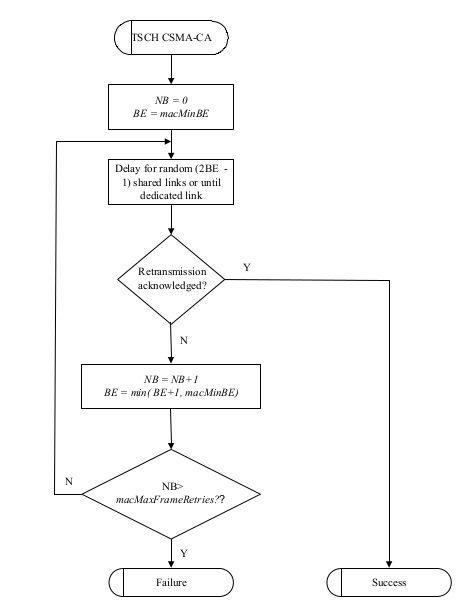
\includegraphics[scale=0.7]{images/tsch_csma_backoff_algo.png}
    \caption{TSCH CSMA-CA Backoff Algorithmus \cite{IEEE802154e}}
    \label{fig:tsch_csma_backoff_algo}
\end{figure}
